\documentclass[dvipdfmx,cjk]{beamer} 
%\documentclass[dvipdfm,cjk]{beamer} %% オプションは環境や利用するプログラムに
%\documentclass[dvips,cjk]{beamer}   %% よって変える

\AtBeginDvi{\special{pdf:tounicode 90ms-RKSJ-UCS2}} %% しおりが文字化けしないように
%\AtBeginDvi{\special{pdf:tounicode EUC-UCS2}}

%\setbeamertemplate{navigation symbols}{} %% 右下のアイコンを消す

%\usetheme{CambridgeUS}         %% theme の選択
%\usetheme{Boadilla}           %% Beamer のディレクトリの中の
\usetheme{Madrid}             %% beamerthemeCambridgeUS.sty を指定
%\usetheme{Antibes}            %% 色々と試してみるといいだろう
%\usetheme{Montpellier}        %% サンプルが beamer\doc に色々とある。
%\usetheme{Berkeley}
%\usetheme{Goettingen}
%\usetheme{Singapore}
%\usetheme{Szeged}

%\usecolortheme{rose}          %% colortheme を選ぶと色使いが変わる
%\usecolortheme{albatross}

%\useoutertheme{shadow}                 %% 箱に影をつける
%\usefonttheme{professionalfonts}       %% 数式の文字を通常の LaTeX と同じにする

%\setbeamercovered{transparent}         %% 消えている文字をうっすらと表示する
\usepackage{bxdpx-beamer}
\usepackage{pxjahyper}
\usepackage{minijs}
\usepackage{mathrsfs}
\usepackage{amsmath,amsfonts,amsthm,amssymb}
\usepackage{color}
\usepackage{graphics}
\usepackage{tikz}
\usepackage{bm,bbm}
\usepackage{picture}
\usepackage{fancybox}
\usepackage[bold]{otf}
\usepackage{here}
%定理環境の設定
%\usepackage{amsthm}
\theoremstyle{definition}
%\setbeamertemplate{theorems}[numbered] % 定理などに番号をふるために必要 %
\newtheorem{rem}{\textbf{ 注意 }}
\newtheorem{ex}{\textbf{ 例 }}
\newtheorem{dfn}{\textbf{ 定義 }}
\newtheorem{thm}[dfn]{\textbf{ 定理 }}
\newtheorem{prop}[dfn]{\textbf{ 命題 }}
\newtheorem{lem}[dfn]{\textbf{ 補題 }}
\newtheorem{cor}[dfn]{\textbf{ 系 }}
\newtheorem{axi}[dfn]{\textbf{ 公理 }}
\renewcommand{\proofname}{\textbf{証明}}




%スタイルファイルを追加したい場合は以下のように書く
\usepackage{graphicx}
\usepackage{amsmath,amssymb}
%\usepackage{eclbkbox}
\usepackage{tikz}

%\newcommandでマクロを定義できる
\newcommand{\macrotest}{\LaTeX のマクロは便利}
\newcommand{\PD}[2]{\frac{\partial {#1}}{\partial {#2}}}%引数もとれる
\newcommand{\combination}[2]{{}_{#1} \mathrm{C}_{#2}}

\begin{document}
\title[多様体の次元を調べる方法]{多様体の次元を調べる方法} 
\author[青見健志]{青見健志}            %% ここに書かれた情報は色々なところに使われるので
\institute[空間数理研究室]{空間数理研究室}   %% なるべく設定した方が良い
\date{令和6年2月8日}

\begin{frame}                  %% \begin{frame}..\end{frame} で 1 枚のスライド
\titlepage                     %% タイトルページ
\end{frame}

\begin{frame}                  %% 目次 (必要なければ省略)
\tableofcontents
\end{frame}

\section{はじめに}
\begin{frame}
\frametitle{はじめに} 
どこでも好きなところに$m$次元の局所座標系
を描ける空間を$m$次元多様体という. 例えば, 球面
は球面上のどこでも好きなところに
$2$次元の局所座標系を描くことができるため, 
$2$次元多様体である.  

私は複雑な方程式で表された空間や
高次元の空間などの形を理解することに興味をもち, 
多様体の次元を調べる方法を研究することにした. 
  \begin{figure}[]
    \centering
    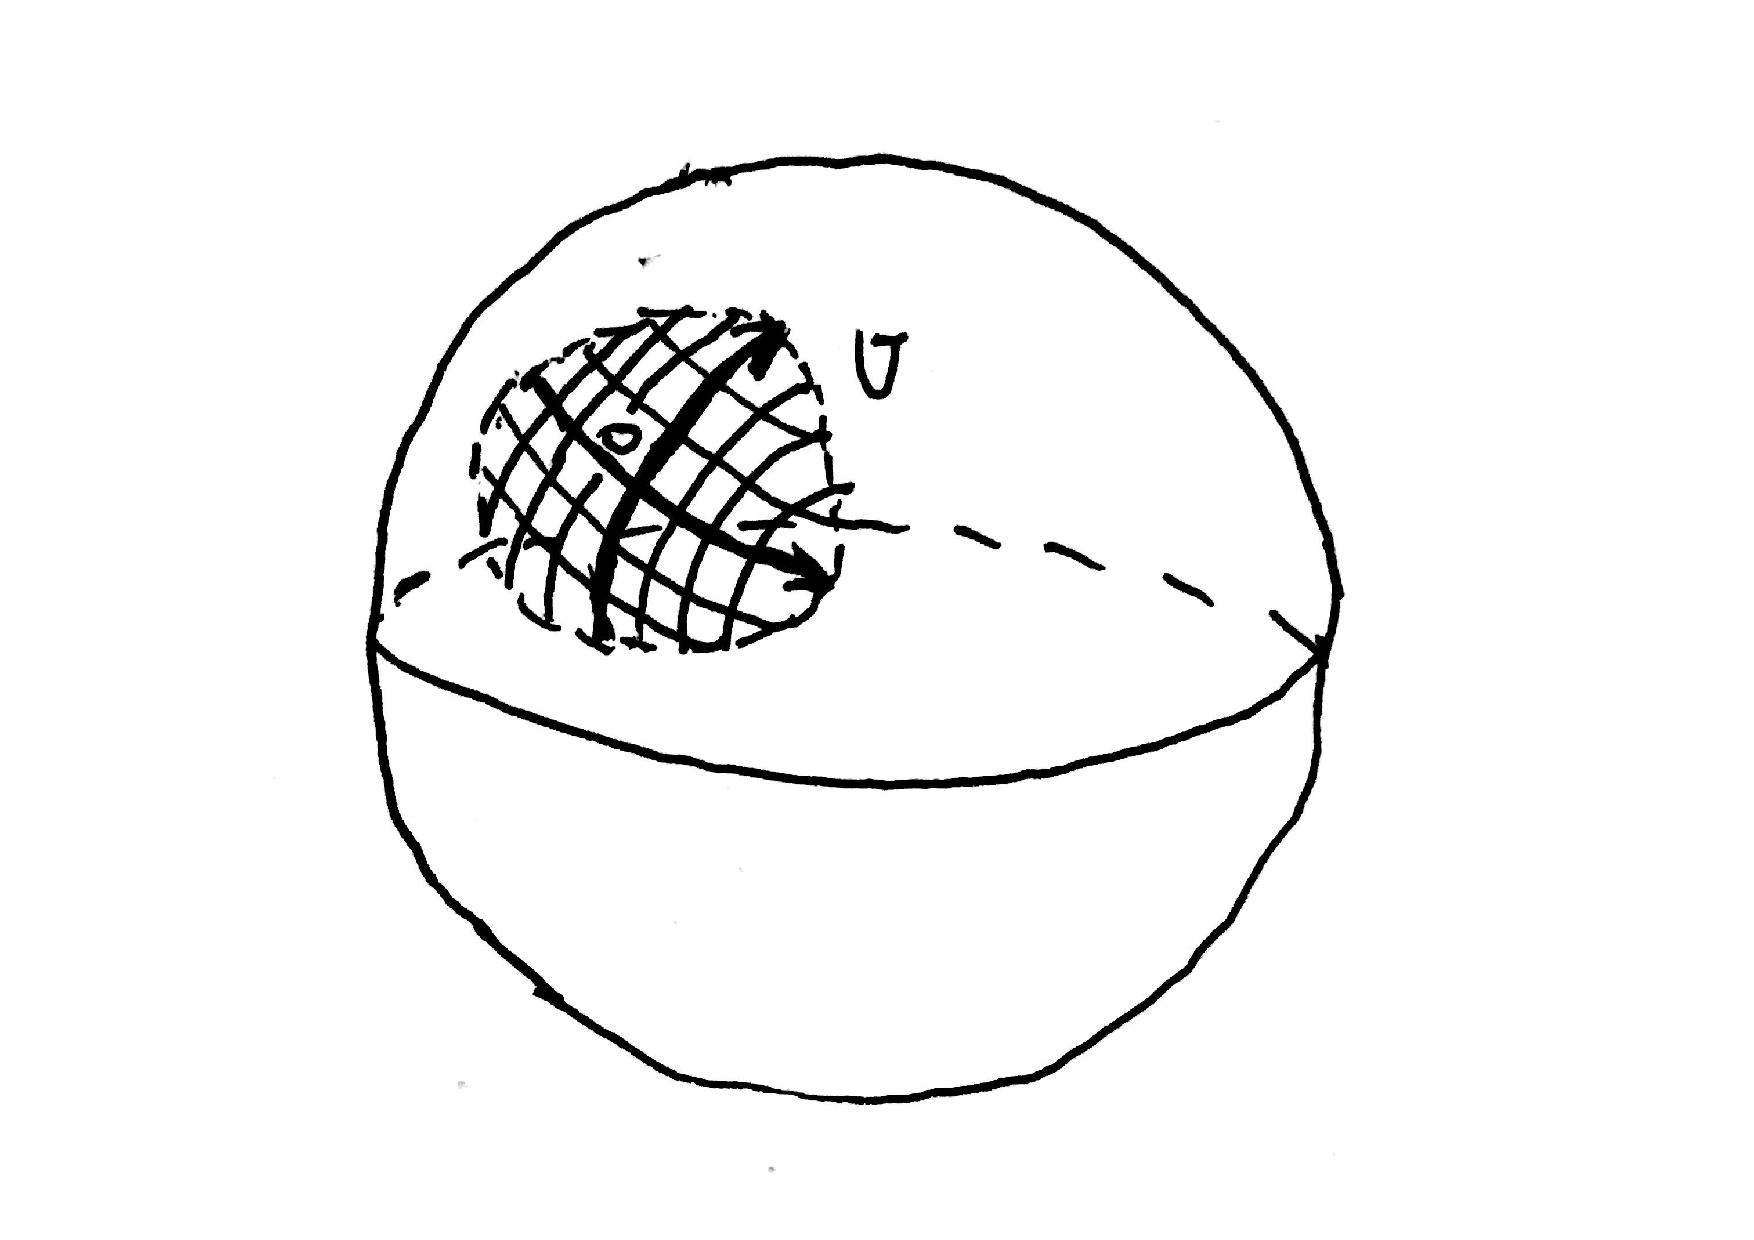
\includegraphics[keepaspectratio, scale=0.2]
         {CoSysInS2.pdf}
    \caption{球面に描かれた局所座標系}
    \label{CoSysInS2}
   \end{figure}
\end{frame}

\begin{frame}
\frametitle{準備} 
\begin{dfn}
位相空間$X$の開集合$U$から, $m$次元数空間$\mathbb{R}^m$のある開集合$U'$
への同相写像
$\varphi : U\rightarrow U'$
があるとき$(U, \varphi)$を$m$次元座標近傍という. 
$\varphi$を$U$上の局所座標系という.
\end{dfn}
\begin{figure}[H]
  \begin{tabular}{cc}
    %---- 最初の図 ---------------------------
    \begin{minipage}[t]{0.45\hsize}
      \centering
      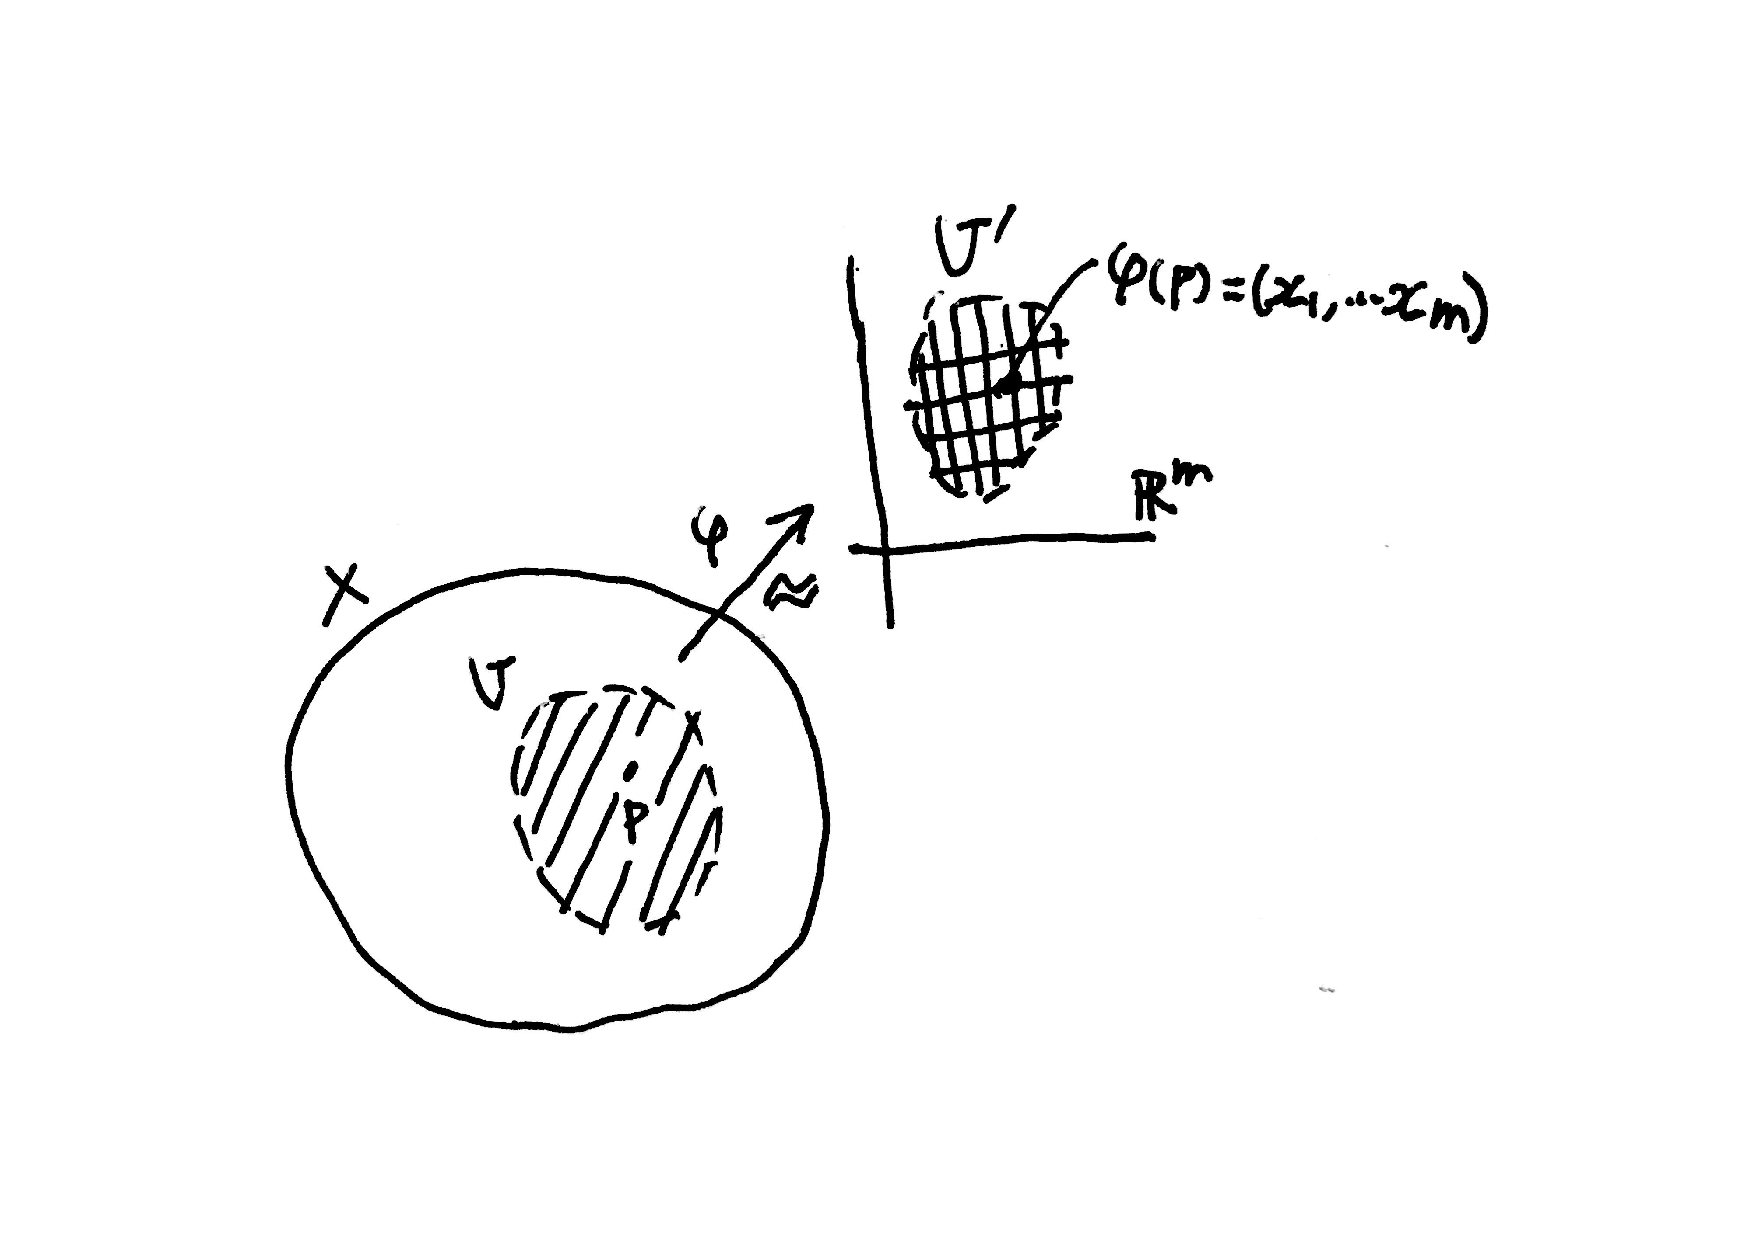
\includegraphics[keepaspectratio, scale=0.2]{coNeighborhoodBig.pdf}
      \caption{$U$上の局所座標系}
      \label{}
    \end{minipage} &
    %---- 2番目の図 --------------------------
    \begin{minipage}[t]{0.45\hsize}
      \centering
      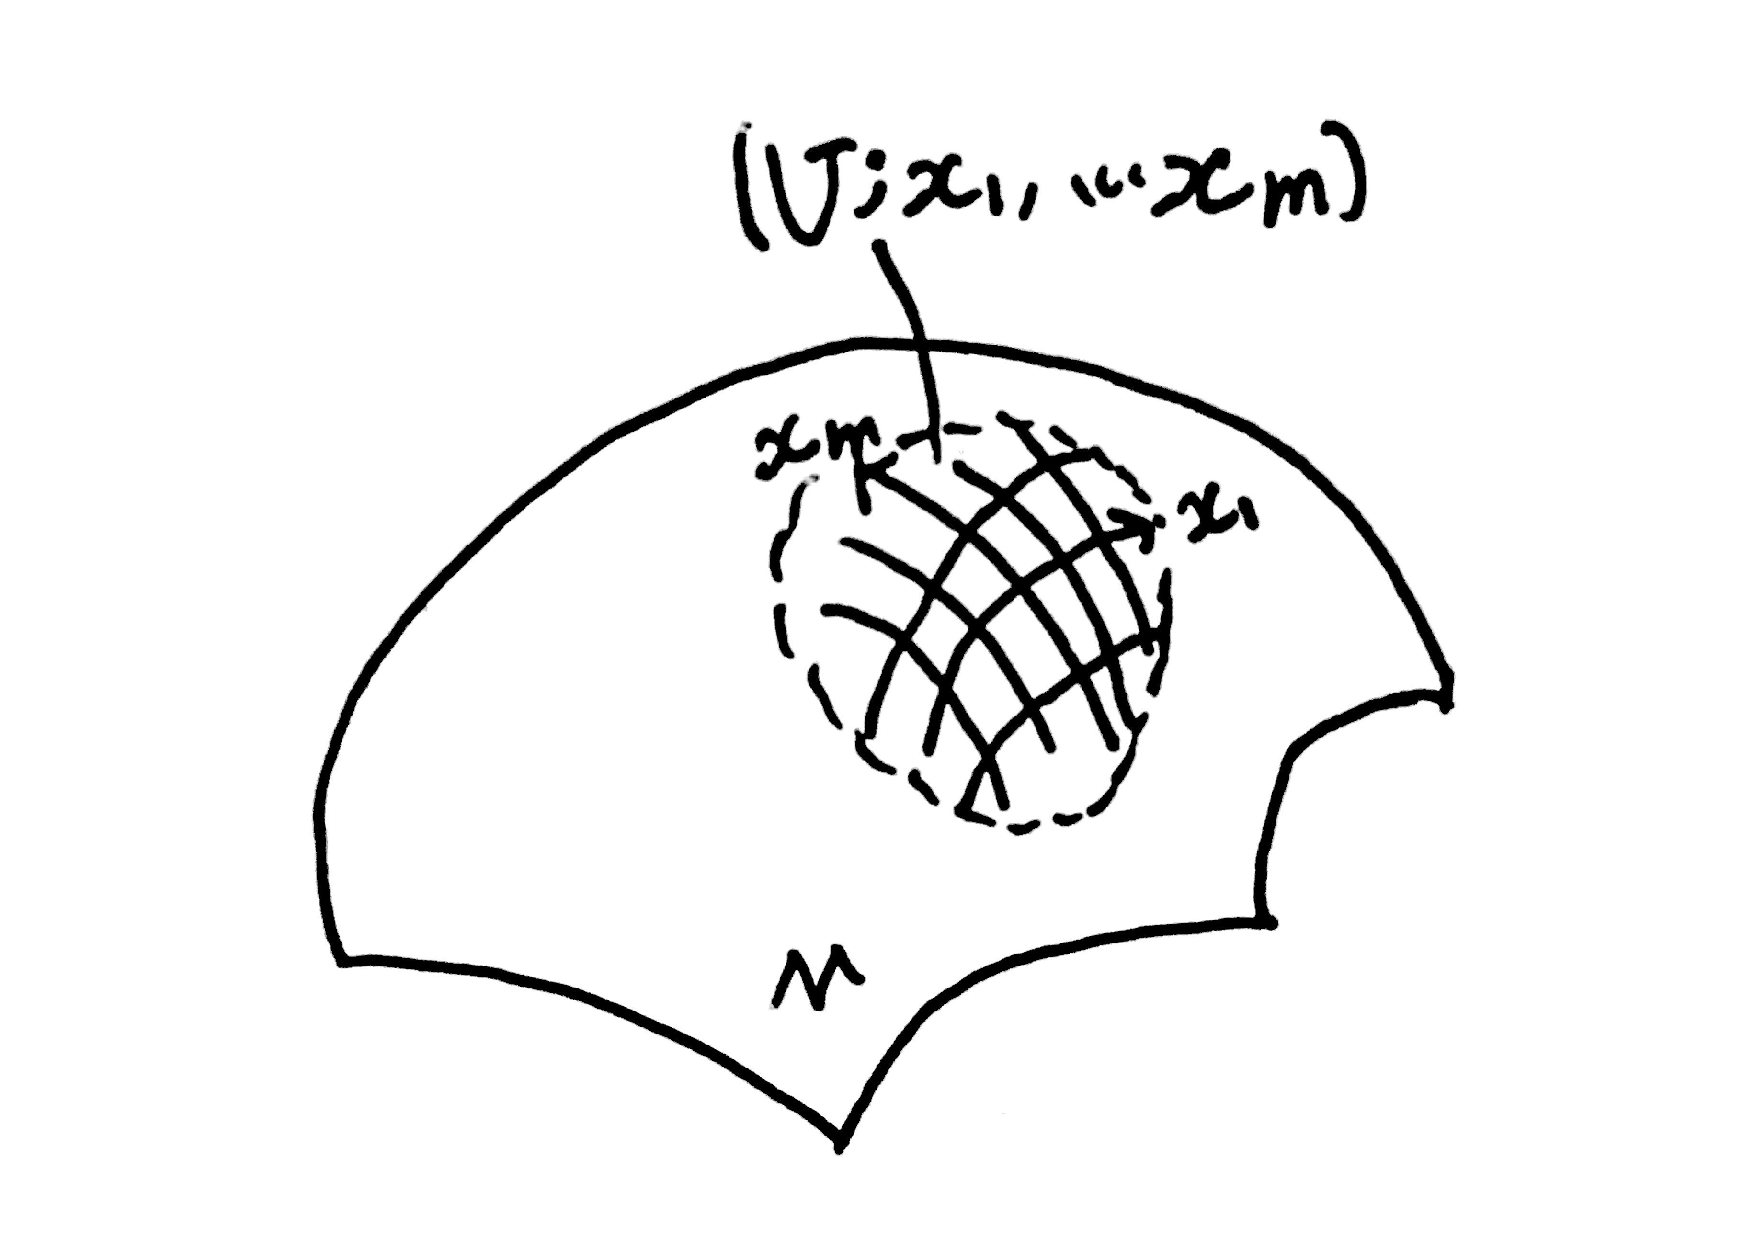
\includegraphics[keepaspectratio, scale=0.2]{DrawnLocalCoSysBig.pdf}
      \caption{局所座標系が描かれていると考える}
      \label{}
    \end{minipage}
    %---- 図はここまで ----------------------
  \end{tabular}
\end{figure}
\end{frame}
\begin{frame}
  \frametitle{}
  \begin{dfn}
    $m$次元位相多様体$M$の$2$つの座標近傍$(U, \varphi)$, 
    $(V, \psi)$が交わっているとき, 同相写像
    $$\psi \circ \varphi^{-1}:\varphi(U\cap V)\rightarrow \psi(U\cap V)$$
    を$(U, \varphi)$から$(V, \psi)$への座標変換という. 
\end{dfn}
座標変換$\psi \circ \varphi^{-1}$の微分可能性は
座標近傍の張り合わせの「滑らかさ」と考えられる. 
\begin{figure}[H]
    \centering
    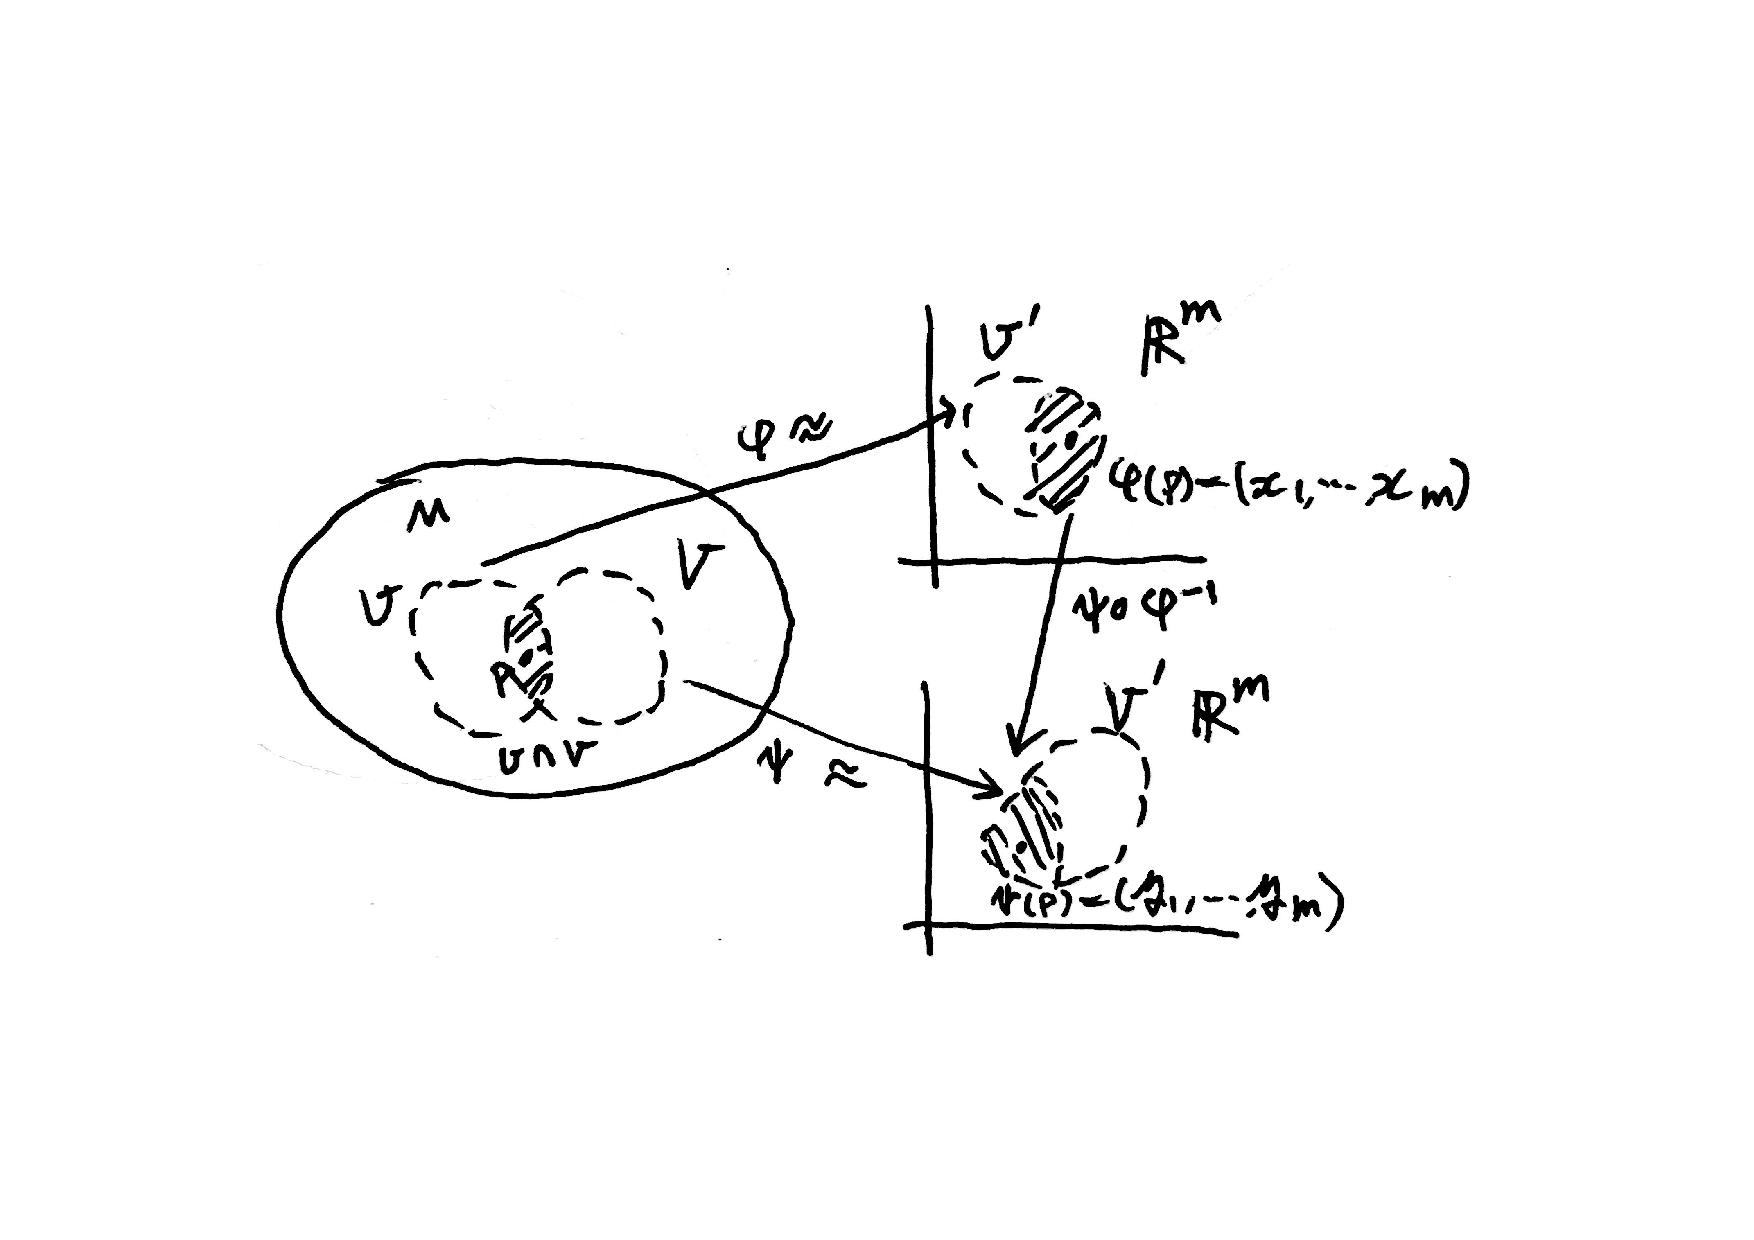
\includegraphics[keepaspectratio, scale=0.3]{coordinateConversionBig.pdf}
    \caption{座標変換$\psi \circ \varphi^{-1}$}
    \label{coordinateConversion}
   \end{figure}
\end{frame}
% \begin{frame}
% \begin{ex}
% $\mathbb{R}^3$内の位相空間としての球面$S^2$の開集合$U_3^+$と
% $\varphi_3^+ : U_3^+ \rightarrow \mathbb{R}^2$をそれぞれ\\
% $U_3^+ = \{(x_1, x_2, x_3)\in S^2|x_3>0\}$\\
% $\varphi_3^+(x_1, x_2, x_3)=(x_1, x_2)$\\
% とすると$(U_3^+, \varphi_3^+)$は$2$次元座標近傍になる. 
% \end{ex}
% \end{frame}

% \begin{frame}
% \begin{proof}
% $\varphi_3^+(U_3^+)=\{(x_1,x_2)\in \mathbb{R}^2|x_1^2+x_2^2<1\}$より, 
% $\varphi_3^+$は$S^2$の開集合から$\mathbb{R}^2$の開集合への写像になっている. \\
% また, $\varphi_3^+(x_1, x_2, x_3)=(x_1, x_2)$より, $\varphi_3^+$は全単射かつ連続である. \\
% さらに, $\varphi_3^+$の逆関数$(\varphi_3^+)^{-1}$は
% $(\varphi_3^+)^{-1}(x_1,x_2)=\left(x_1,x_2,\sqrt{1-(x_1^2+x_2^2)} \right)$となり, これも連続である, 
% よって, $(U_3^+, \varphi_3^+)$は$2$次元座標近傍になる. 
% \end{proof}
% \begin{tikzpicture}[scale=1.2]
% \draw[->,>=stealth,semithick] (-2,0)--(2,0) node[right]{$x_1$}; %x軸
% \draw[->,>=stealth,semithick] (0,-2)--(0,2) node[left]{$x_3$}; %y軸
% \draw[->,>=stealth,semithick] (-2,-0.5)--(1.5,0.5) node[left]{$x_2$}; %y軸
% \draw (0,0) node[below left]{O}; %原点
% \draw (1.5,0) arc (0:180:1.5);
% \draw[dashed](0,0)circle[x radius=1.5,y radius=0.5];
% \draw[->,thick](-0.7,1)--(-0.7,-0.1);
% \node at(1.2,1.2) {$U_3^+$};
% \node at(-0.4,1){$\varphi_3^+$};
% \end{tikzpicture}

% \end{frame}

\begin{frame}
  \frametitle{準備} 
  \begin{dfn}
  $r$を自然数または$\infty$とする. 位相空間$M$が条件(1), (2), (3)をみたすとき, 
  $M$を$m$次元$\mathit{C}^r$級多様体という. \\
  (1)$M$はハウスドルフ空間である. \\
  (2)$M$は$m$次元座標近傍によって被覆される. \\
  (3)$U_\alpha \cap U_\beta \neq \phi$であるような座標近傍$(U_\alpha, \varphi_\alpha)$, 
  $(U_\beta, \varphi_\beta)$について座標変換
  $$\varphi_\beta \circ \varphi_\alpha^{-1}: \varphi_\alpha(U_\alpha \cap U_\beta)
  \rightarrow \varphi_\beta(U_\alpha \cap U_\beta)$$
  は$\mathit{C}^r$級写像である. 
  \end{dfn}
  \end{frame}
  
  \section{多様体の例}
  \begin{frame}
  \begin{thm}
    $m$次元球面$S^m \in \mathbb{R}^{m+1}$を
    $$S^m=\{(x_1,\cdots x_{m+1})|x_1^2+\cdots +x_{m+1}^2=1\}$$
    と定義すると, $S^m$は$m$次元$C^{\infty}$級多様体である. 
  \end{thm}
  \ \\
  \ \\
  \ \\
    \begin{tikzpicture}[scale=1]
      % 球面の描画
      \draw (0, 0, 0) circle (1);
        % 下半分の楕円の描画
      \draw[dashed] (0, 0) ellipse (1 and 0.3);
  % 2点の座標
      \coordinate (A) at (-0.23-0.04, -0.75);
      \coordinate (B) at (-0.02-0.04, 0.8);
     \coordinate (C) at (-1, 0);
      \coordinate (D) at (0.8, 0);
      
      % 曲線の描画
      \draw[line width=1pt,->] (A) to[bend left] (B);
      \draw[line width=1pt,->] (C) to[bend left] (D);
      
  \node at (0.27, 0.5)  {{\fontsize{9pt}{12pt}\selectfont $(U_i^{\pm}, \varphi_i^{\pm})$}};
  \node at (-1, 0.75)  {$S^2$};
  \end{tikzpicture}

\end{frame}
  \begin{frame}
    $\mathbb{R}^{m+1}$はハウスドルフ空間
        であるから, その部分空間として, $S^m$は
        ハウスドルフ空間である. 
        $S^m$の$2(m+1)$個の開集合
        $U_i^+$, $U_i^-$ $(i=1,\cdots ,m+1)$を
        次のように定義する. 
        $$U_i^+ = \{(x_1, \cdots x_i, \cdots ,x_{m+1})\in S^m|x_i>0\}$$
        $$U_i^- = \{(x_1, \cdots x_i, \cdots ,x_{m+1})\in S^m|x_i<0\}$$
        $S^m$はこれら$U_i^+$, $U_i^-$ $(i=1,\cdots ,m+1)$
        で被覆される. 写像$\varphi_i^+:U_i^+ \rightarrow \mathbb{R}^m$, 
        $\varphi_i^-:U_i^- \rightarrow \mathbb{R}^m$を
        それぞれ次のように定義する. 
        $$\varphi_i^+(x_1,\cdots ,x_i,\cdots, x_{m+1})=(x_1,\cdots ,\hat{x_i},\cdots ,x_{m+1})$$
        $$\varphi_i^-(x_1,\cdots ,x_i,\cdots, x_{m+1})=(x_1,\cdots ,\hat{x_i},\cdots ,x_{m+1})$$
        ここで, $\hat{x_i}$は$x_i$を取り去るという意味である. 
      \end{frame}
  \begin{frame}
    \begin{figure}[H]
      \begin{tabular}{cc}
        %---- 最初の図 ---------------------------
        \begin{minipage}[t]{0.45\hsize}
          \centering
          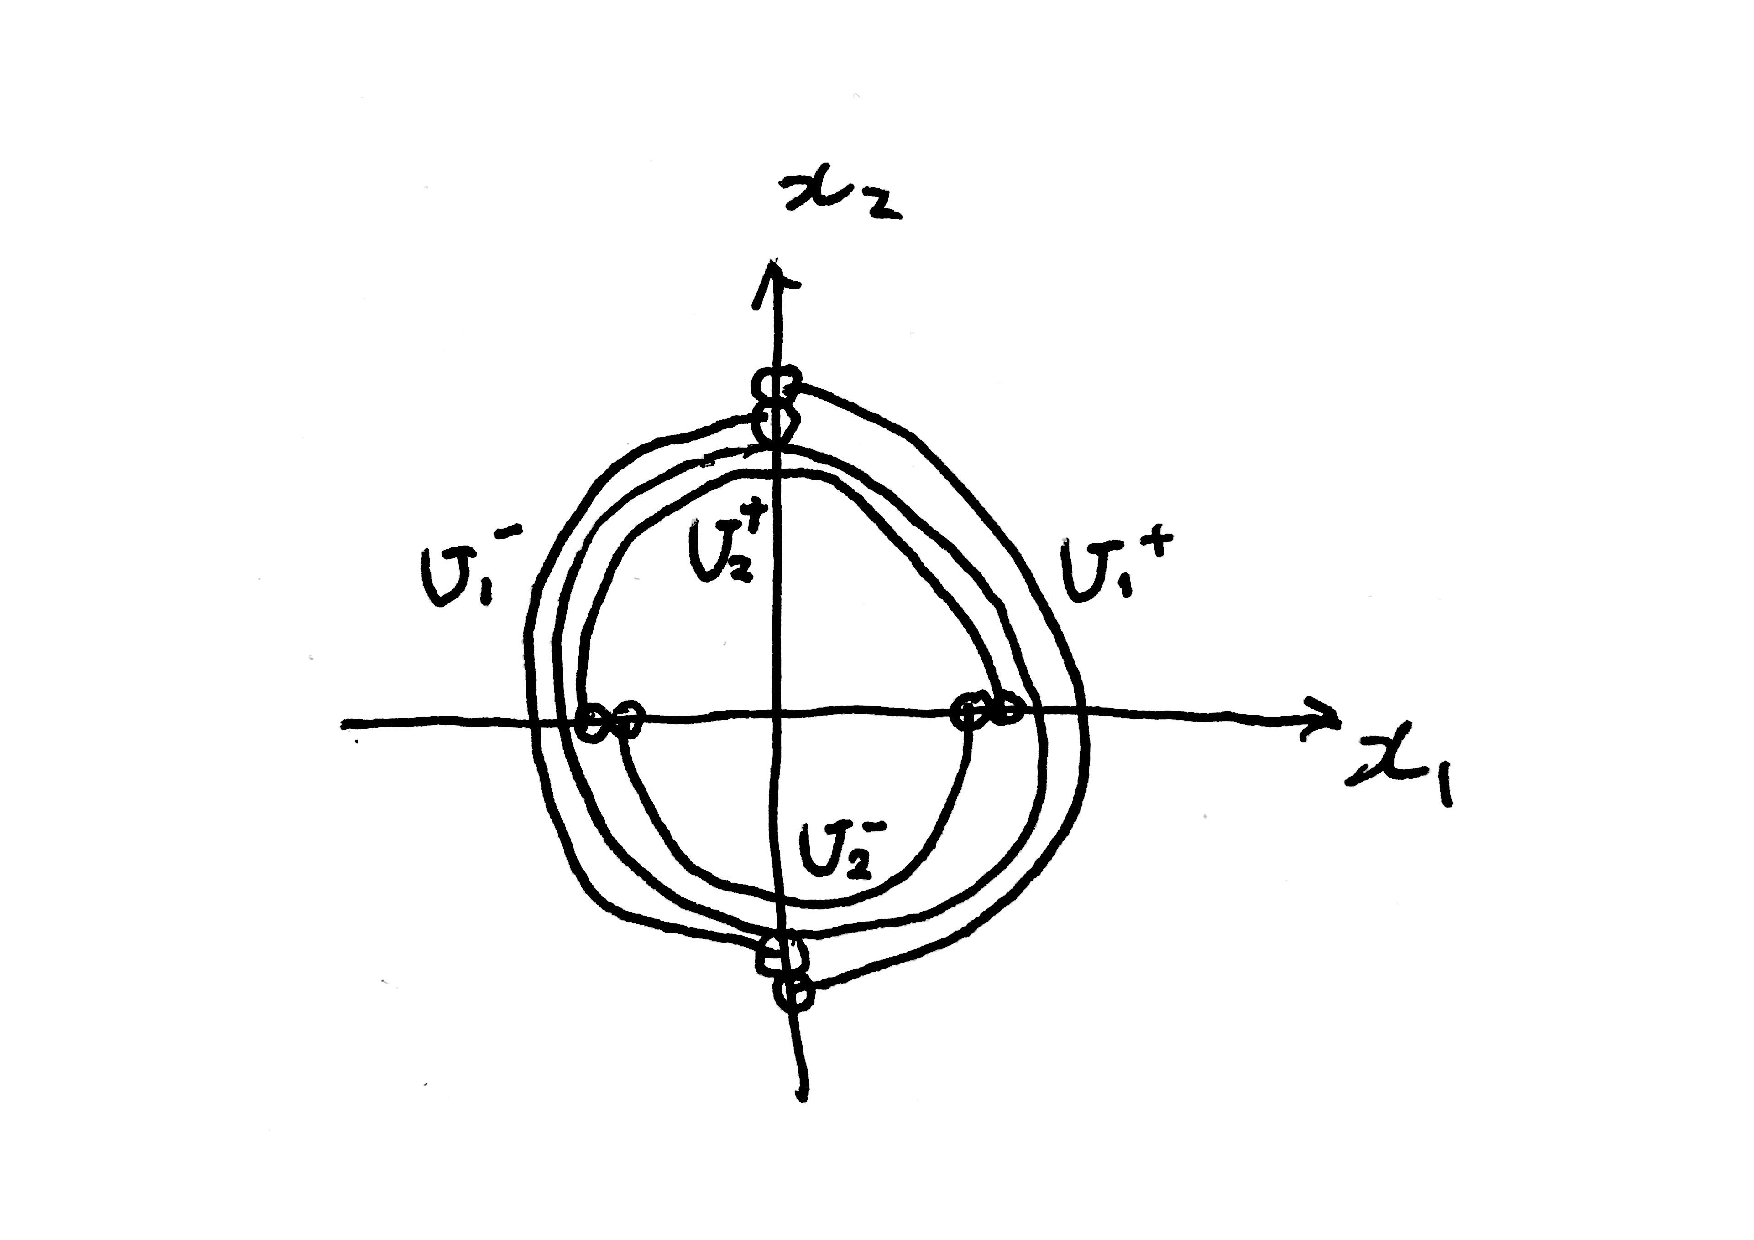
\includegraphics[keepaspectratio, scale=0.25]{localCoSysOfS1_1.pdf}
          \caption{$S^1$の開集合}
          \label{}
        \end{minipage} &
        %---- 2番目の図 --------------------------
        \begin{minipage}[t]{0.45\hsize}
          \centering
          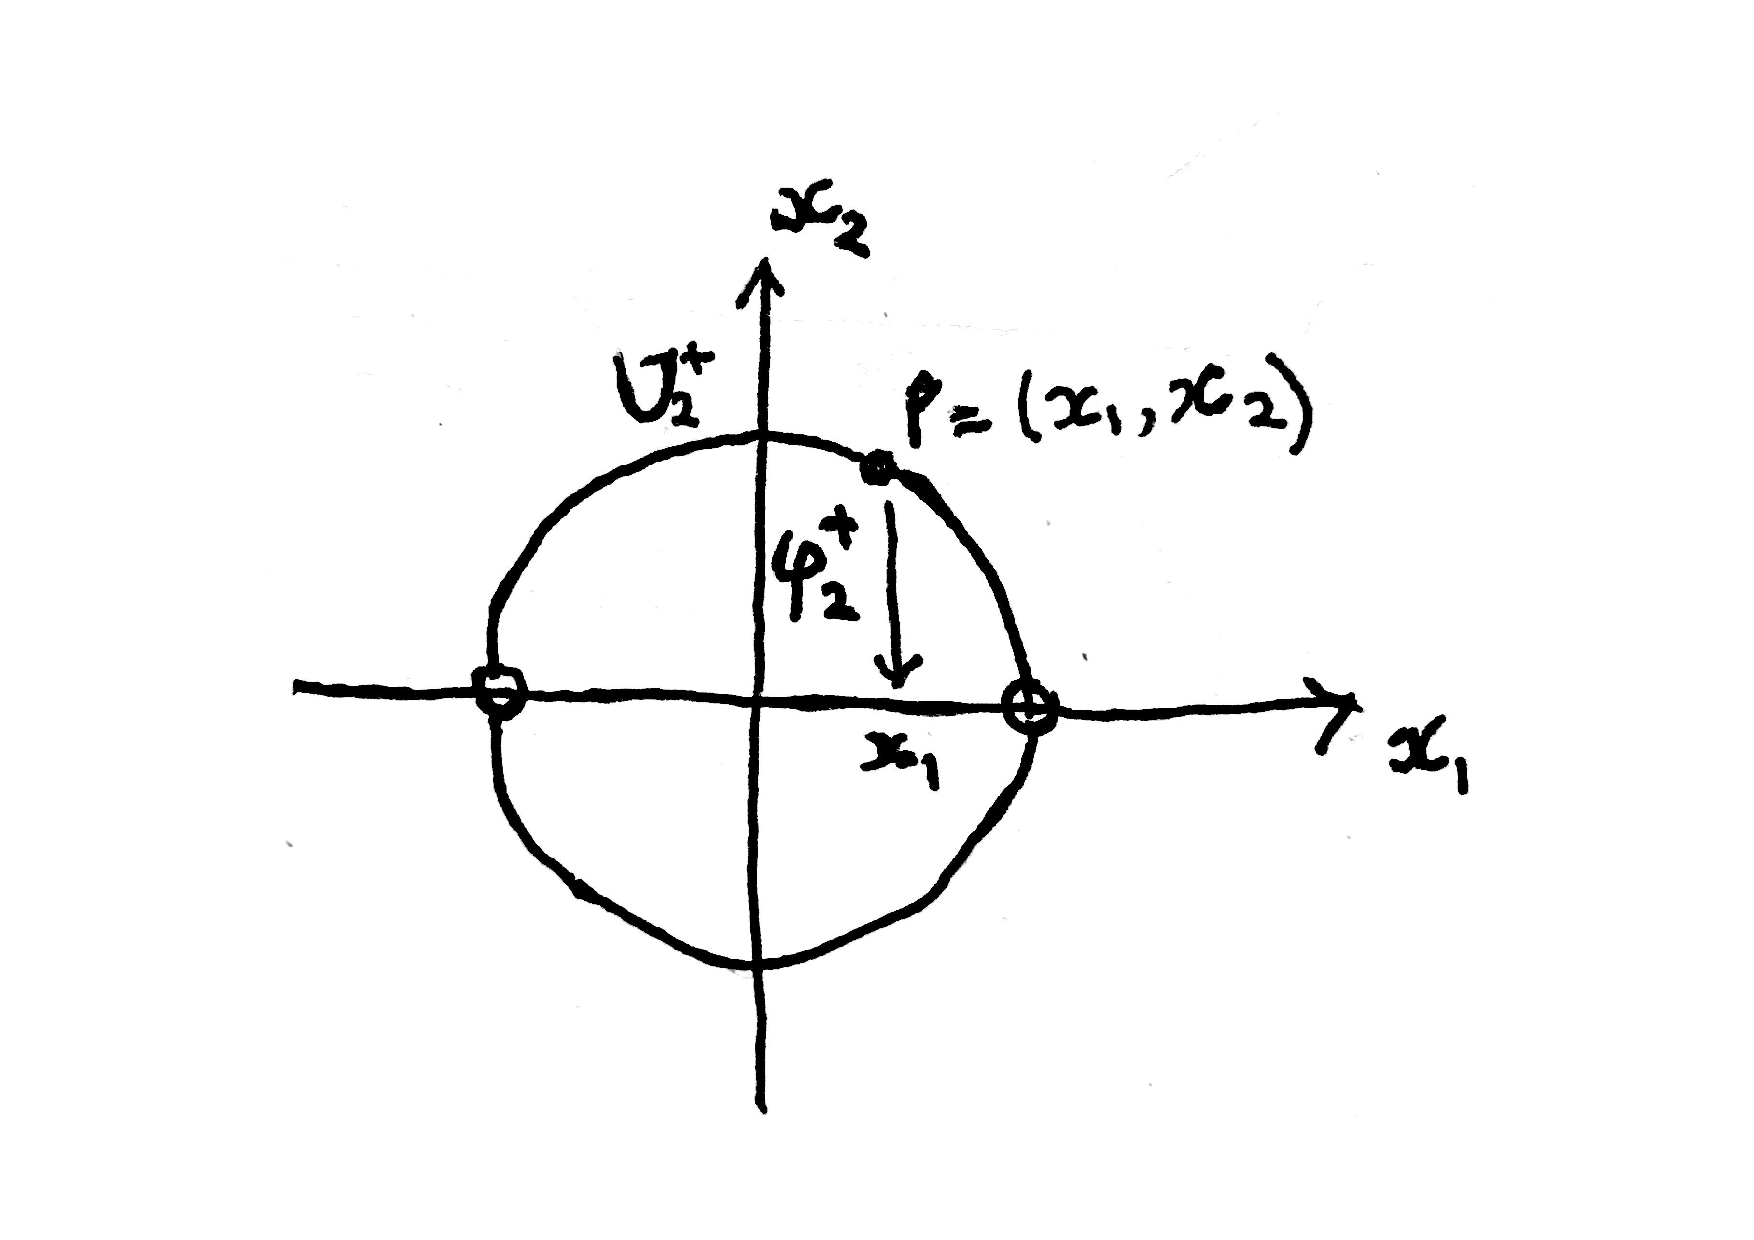
\includegraphics[keepaspectratio, scale=0.25]{localCoSysOfS1_2.pdf}
          \caption{$S^1$の局所座標系}
          \label{}
        \end{minipage}
        %---- 図はここまで ----------------------
      \end{tabular}
    \end{figure}

        このとき, 
        $\varphi_i^+$, $\varphi_i^-$はそれぞれ, $U_i^+$, 
        $U_i^-$から$\mathbb{R}^m$への射影であるから, 同相写像であり, 
        すべての座標変換$\varphi_b^+\circ(\varphi_a^+)^{-1}\ 
        (1\leq a, b\leq 2(m+1))$が$C^{\infty}$級であることが確かめられる. 
        よって, $S^m$は$m$次元$C^{\infty}$級多様体であることがわかる. 
\end{frame}

\begin{frame}
  \begin{dfn}\label{def:C^s map}
    連続写像$f:M\to N$が$1$点$p\in M$において
    $C^s$級であるとは, $p$を含む$M$の$C^r$級
    座標近傍$(U,\varphi)$と
    $f(p)$を含む$N$の
    座標近傍$(V,\psi)$が存在して, 
    \begin{itemize}
        \item[(1)]$f(U)\subset V$
        \item[(2)]$(U,\varphi)$と
        $(V,\psi)$に関する$f$の
        局所座標表示
        $\psi\circ f\circ \varphi^{-1}$
        が$C^s$級である.
        (ただし, $0\leq s \leq r \leq \infty$) 
    \end{itemize}
    この$2$つの条件が成り立つことである. 
    $f$が任意の点$p\in M$で$C^s$級であるとき, 
    $f$は$C^s$級写像であるという. 
  \end{dfn}
  \begin{figure}[H]
    \centering
    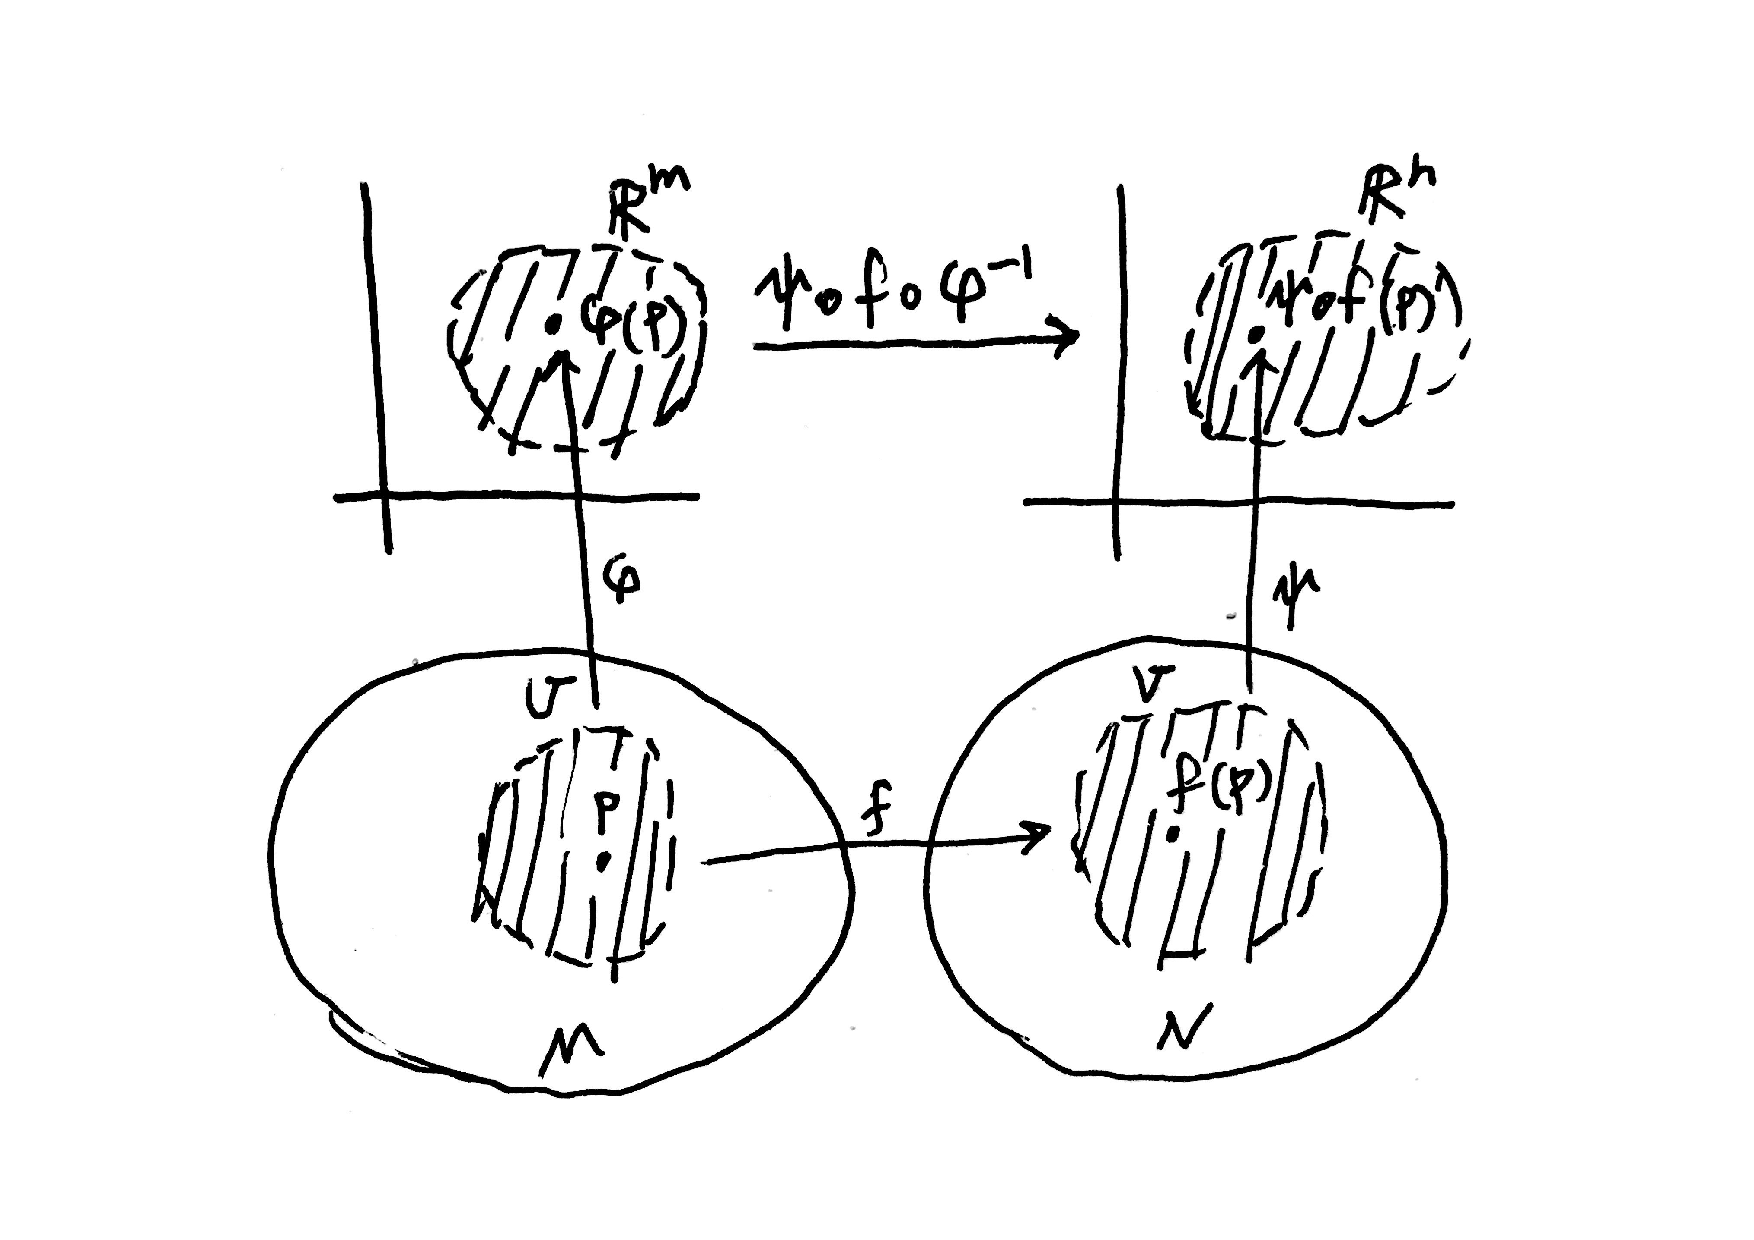
\includegraphics[keepaspectratio, scale=0.2]
         {Csmap.pdf}
    \caption{$f$と$\psi\circ f\circ \varphi^{-1}$
    の関係}
    \label{Csmap}
  \end{figure}
\end{frame}

\begin{frame}
  \frametitle{}
  \begin{dfn}
    $p$を含む座標近傍$(U,\varphi)$を
    $1$つ固定する. $p$のまわりで定義された
    $C^r$級関数$f$に, $p$における$x_i$
    方向の偏微分係数を対応させる操作を
    $\left(\frac{\partial}{\partial x_i}
    \right)_p$と書く. すなわち, 
    $$\left(\frac{\partial}{\partial x_i}
    \right)_p:f\mapsto 
    \frac{\partial f\circ \varphi^{-1}}{\partial x_i}(
      \varphi(p))$$
    である. 
  \end{dfn}
\end{frame}

\begin{frame}
  \begin{dfn}\label{def:tangent vector space}
    $m$個のベクトル
    $\left(\frac{\partial}{\partial x_1}\right)_p, 
    \cdots 
    \left(\frac{\partial}{\partial x_m}\right)_p$
    の張るベクトル空間を, 点$p$
    における$M$の接ベクトル空間とよび, 
    $T_p(M)$
    という記号で表す. 接ベクトル空間$T_p(M)$の
    元$\boldsymbol{v}\in T_p(M)$を接ベクトルとよぶ. 
  \end{dfn}
  \begin{figure}[H]
        \centering
        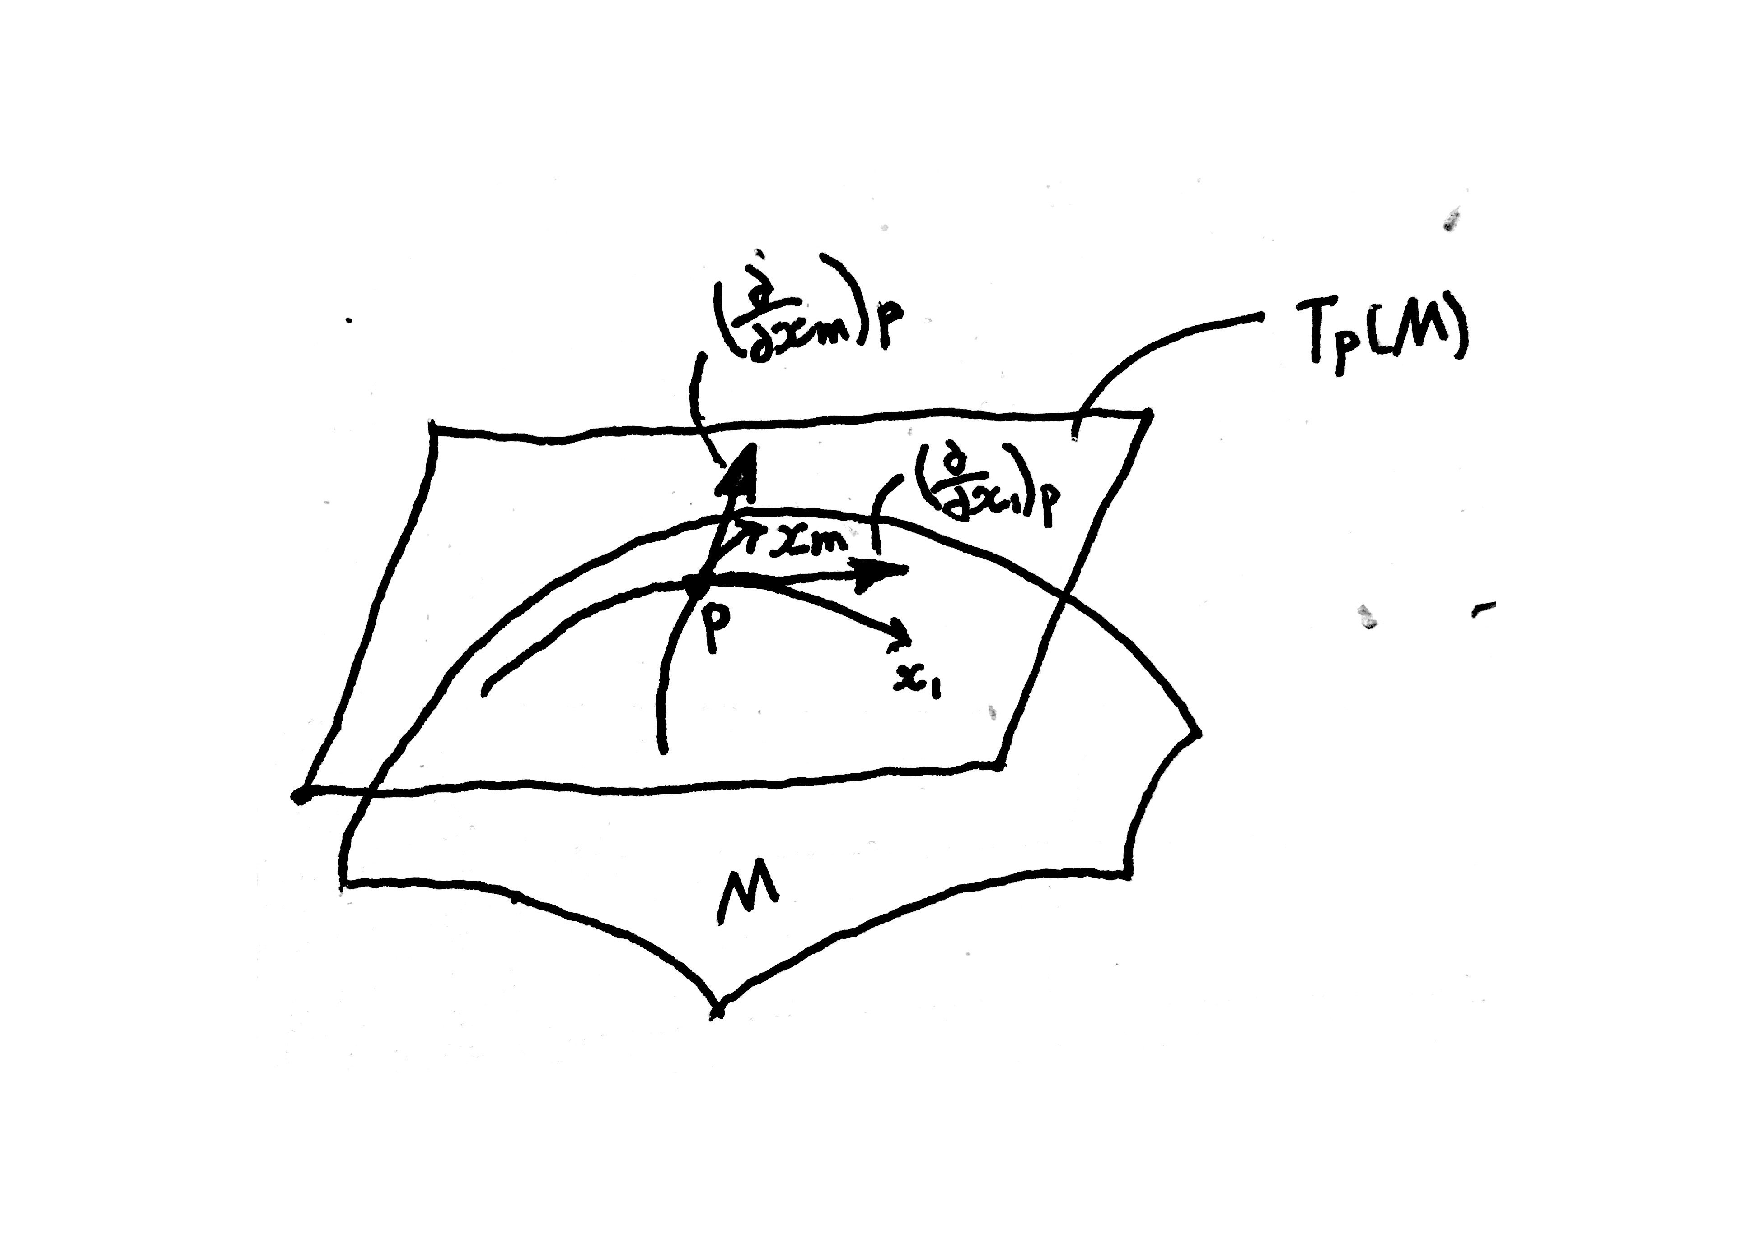
\includegraphics[keepaspectratio, scale=0.28]{tangentVectorSpace_2.pdf}
        \caption{$T_p(M)$のイメージ}
        \label{}
  \end{figure}

\end{frame}
\begin{frame}
  \frametitle{}
  \begin{definition}\label{def:differential}
    任意の接ベクトル$\boldsymbol{v}\in T_p(M)$
    を$\boldsymbol{v}=
    \sum_{i=1}^{m}v_i\left(\frac{\partial}
    {\partial x_i}\right)_p$とし, $m$次元
    数ベクトル$(v_1,\cdots ,v_m)$とみなすとき, 
     $$(df)_p:T_p(M)\to T_{f(p)}(N),\ 
    \begin{pmatrix}
      v_1\\
      \vdots \\
      v_m
    \end{pmatrix}
    \mapsto
    (Jf)_p
    \begin{pmatrix}
      v_1\\
      \vdots \\
      v_m
    \end{pmatrix}$$
    を, 点$p$における$f:M\to N$
    の微分とよぶ. ただし, $(Jf)_p$は
    点$p$におけるヤコビ行列
    $$(Jf)_p=
    \left(
    \begin{array}{ccc}
      \frac{\partial (\psi\circ f\circ \varphi^{-1})_1}{\partial x_1}(\varphi(p))&\cdots &\frac{\partial (\psi\circ f\circ \varphi^{-1})_1}{\partial x_m}(\varphi(p))\\
      \vdots &\ddots& \vdots \\
      \frac{\partial (\psi\circ f\circ \varphi^{-1})_n}{\partial x_1}(\varphi(p))&\cdots &\frac{\partial (\psi\circ f\circ \varphi^{-1})_n}{\partial x_m}(\varphi(p)) 
    \end{array} 
    \right)$$
    であるとする. 
  \end{definition}
\end{frame}
\begin{frame}
  \frametitle{写像の局所的性質}
  \begin{thm}\label{theo: projection theorem}
    $f:M\to N$を$C^r$級写像とする. ある点$p\in M$
    における微分$(df)_p:T_p(M)\to T_p(N)$が上への
    線型写像なら, 点$p$付近での$f$の様子は, 射影:
    $\mathbb{R}^{m-n} \times \mathbb{R}^n \to \mathbb{R}^n$, 
    $(x_1, \cdots ,x_m)\mapsto (x_(m-n+1), \cdots ,x_m)$
    と同じである. すなわち, $f(p)$のまわりの局所座標系
    $(y_1, \cdots ,y_n)$に対して
    $p$のまわりの局所座標系
    $(x_1,\cdots ,x_m)$をうまく選んで, $f$
    の局所座標表示
    $(y_1, \cdots ,y_n)=f(x_1,\cdots,x_m)$が
    \begin{eqnarray*}
        y_1&=&f_1(x_1,\cdots ,x_m)=x_{m-n+1}\\
        &\vdots& \\
        y_n&=&f_n(x_1,\cdots ,x_m)=x_m
    \end{eqnarray*}
    であるようにできる. 
\end{thm}
\end{frame}
\begin{frame}
  \frametitle{}
  \begin{figure}[H]
    \centering
    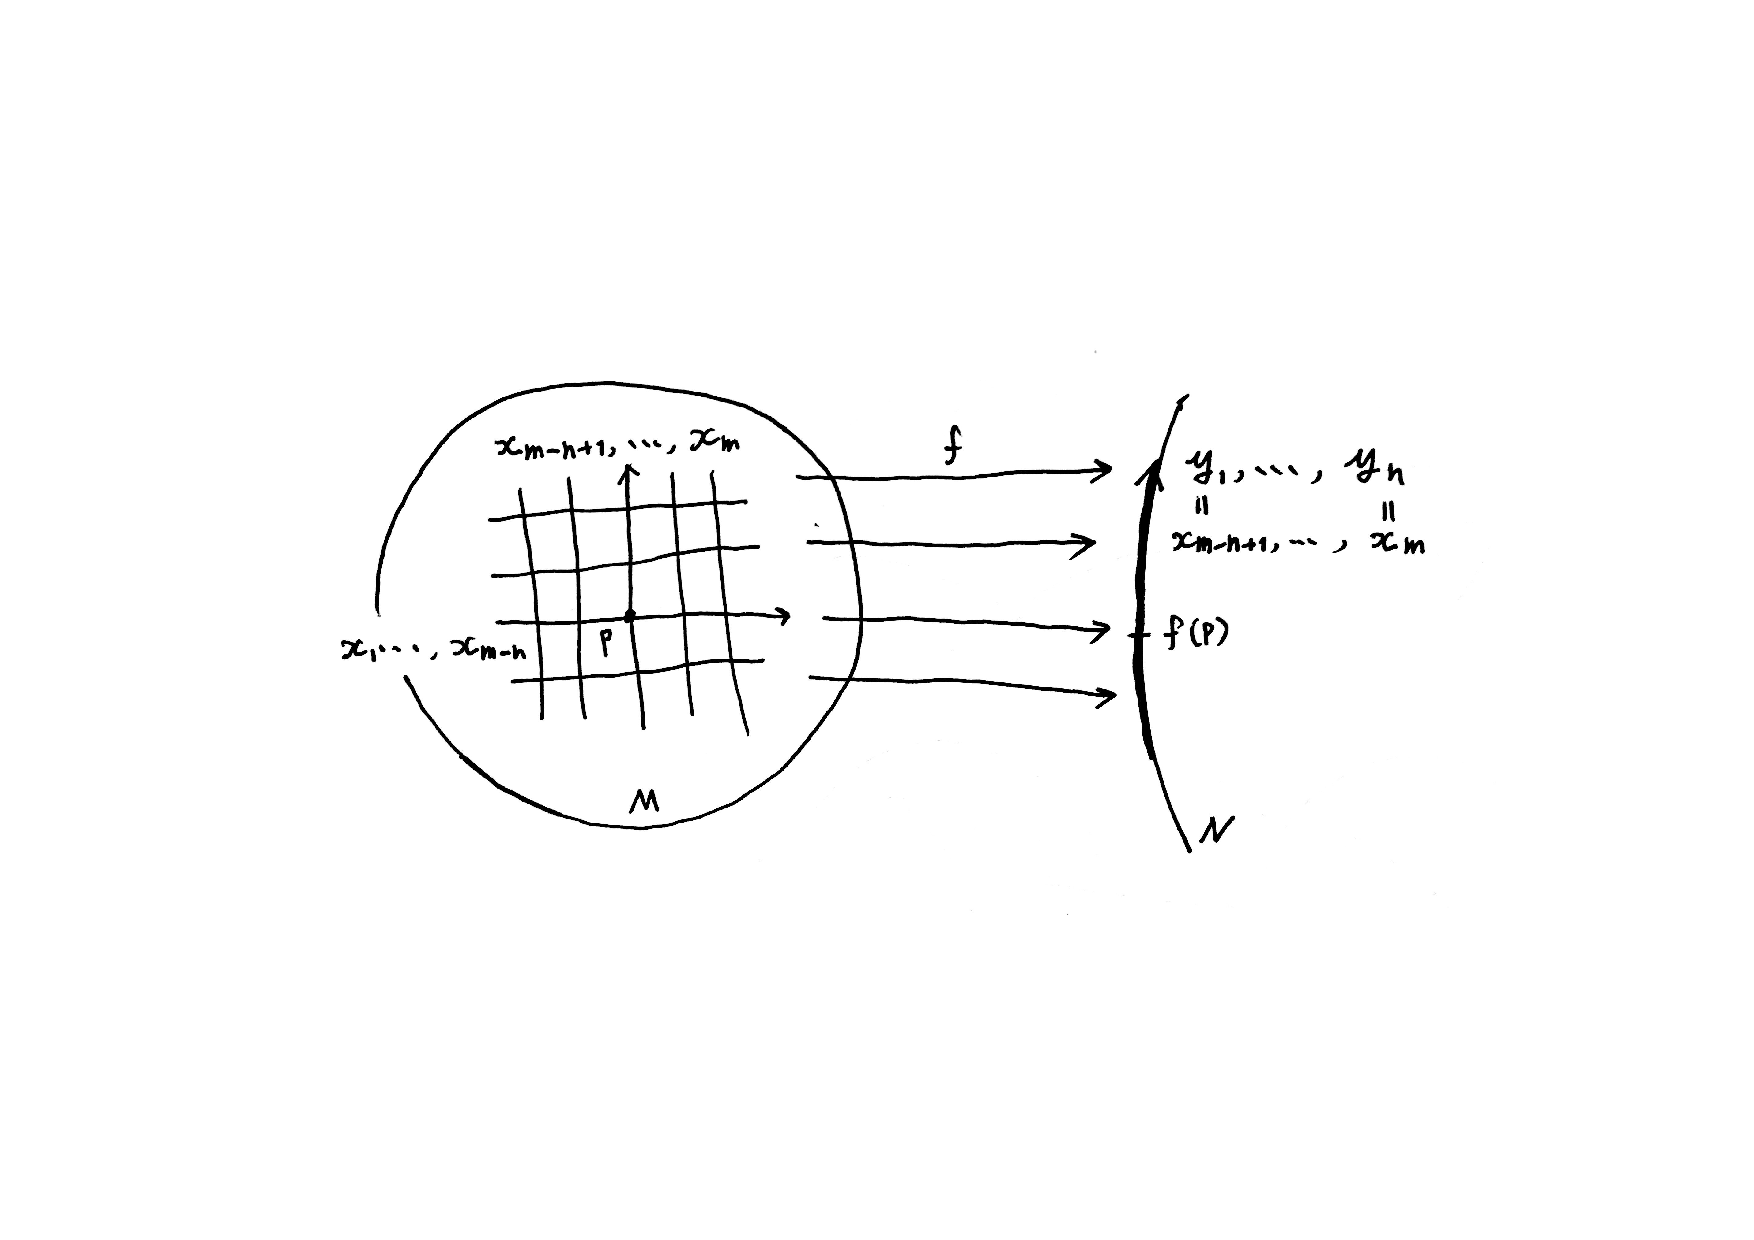
\includegraphics[keepaspectratio, scale=0.5]{projectionTheorem.pdf}
    \caption{射影の様子}
    \label{projectionTheorem}
   \end{figure}
\end{frame}
\begin{frame}
  \frametitle{}
  \begin{definition}\label{def:C^r-submanifold}
    $n$次元$C^r$級多様体$N$の部分集合$L$が
    $N$の$l$次元$C^r$級部分多様体であるとは, 
    \begin{itemize}
        \item[(1)]$l=n$のとき:$L$が$N$の開集合
        であることである. 
        \item[(2)] $0\leq l<n$のとき:$L$の任意の点$p$
        に対し, $p$を含む$N$の座標近傍$(U;x_1,\cdots ,x_n)$
        が存在して, 
        $$L\cap N=\{(x_1,\cdots ,x_n)\in U|
        x_{l+1}=\cdots =x_n=0\}$$
        が成り立つことである. 
    \end{itemize}
\end{definition}
\begin{figure}[H]
    \centering
    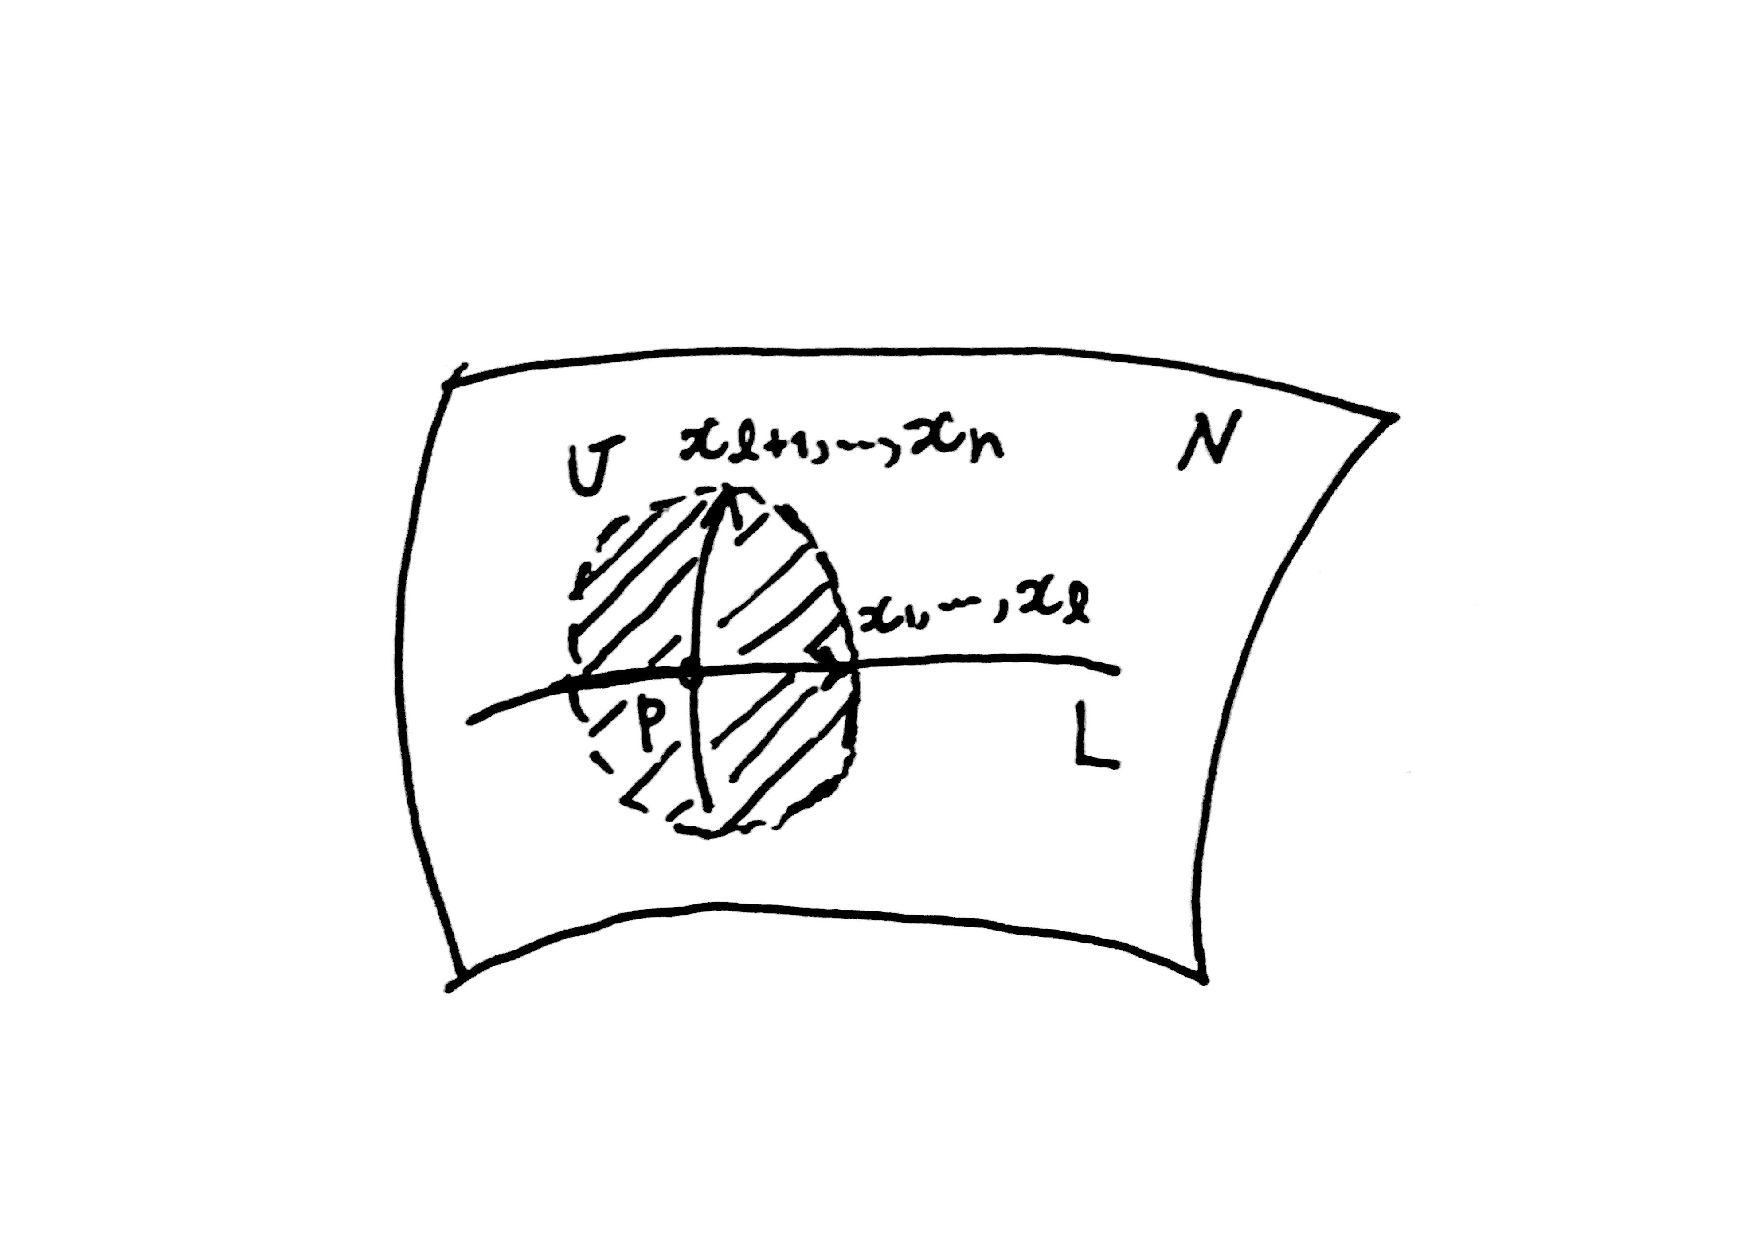
\includegraphics[keepaspectratio, scale=0.2]{CrSubmanifold.pdf}
    \caption{$N$の部分多様体$L$}
    \label{CrSubmanifold}
   \end{figure}
\end{frame}
\begin{frame}
  \frametitle{}
  \begin{prop}\label{prop:dim of C^r-submanifold}
    $n$次元$C^r$級多様体$N$の$l$次元$C^r$級
    部分多様体$L$は, それ自身$l$次元$C^r$級
    多様体である. 
\end{prop}
  

\end{frame}
  \begin{frame}
    \frametitle{}
    \begin{thm}\label{theo:f^{-1}(q) C^r manifold}
      $M$, $N$を$m$次元, $n$次元の$C^r$級多様体, 
      $f:M\to N$を$C^r$級写像とする. $N$のある点
      $q$について, $f(p)=q$となる$M$の各点$p$
      が常にrank$(Jf)_p=n$を満たすとき, 逆像
      $f^{-1}(q)$は$(m-n)$次元$C^r$級多様体
      である. 
    \end{thm}
  \end{frame}

\begin{frame}
  \frametitle{多様体の次元の具体的な計算}
  \begin{ex}
    $n$次元球面
    $$S^n=\{(x_1,\cdots ,x_{n+1}\in 
    \mathbb{R}^{n+1})|x_1^2+\cdots +x_{n+1}^2=1\}$$
    は$n$次元$C^\infty$級多様体である. 
\end{ex}

$C^\infty$級写像($C^\infty$級関数)
$f:\mathbb{R}^{n+1}\to \mathbb{R}$を
$$f(x_1,\cdots ,x_{n+1})=
x_1^2+\cdots +x_{n+1}^2-1$$
で定義すると, 
$S^n=\{(x_1,\cdots ,x_{n+1}\in 
\mathbb{R}^{n+1})|f(x_1,\cdots ,x_{n+1})=0\}
=f^{-1}(0)$
より, $S^n$は逆像$f^{-1}(0)$となっている. 
ヤコビ行列$(Jf)_{\boldsymbol{x}}$を調べると, 
$\boldsymbol{x}\in S^1$のとき, 
$$(Jf)_{\boldsymbol{x}}=(2x_1,\cdots ,2x_{n+1})
\neq \boldsymbol{o}$$
となり, $(Jf)_{\boldsymbol{x}}$の階数は$1$となる. 
よって, $S^n$は$(n+1)-1=n$次元$C^\infty$級
多様体である. 
\end{frame}
\begin{frame}
  \frametitle{}
  \begin{ex}
    $2$次元トーラス
    $$T^2=S^1\times S^1=
    \{T^2=(x,y,z)\in \mathbb{R}^3|
    (\sqrt{x^2+y^2}-R)^2+z^2=r^2\} $$
    $(0<r<R)$は$2$次元$C^\infty$級多様体である. 
    \begin{figure}[H]
      \centering
      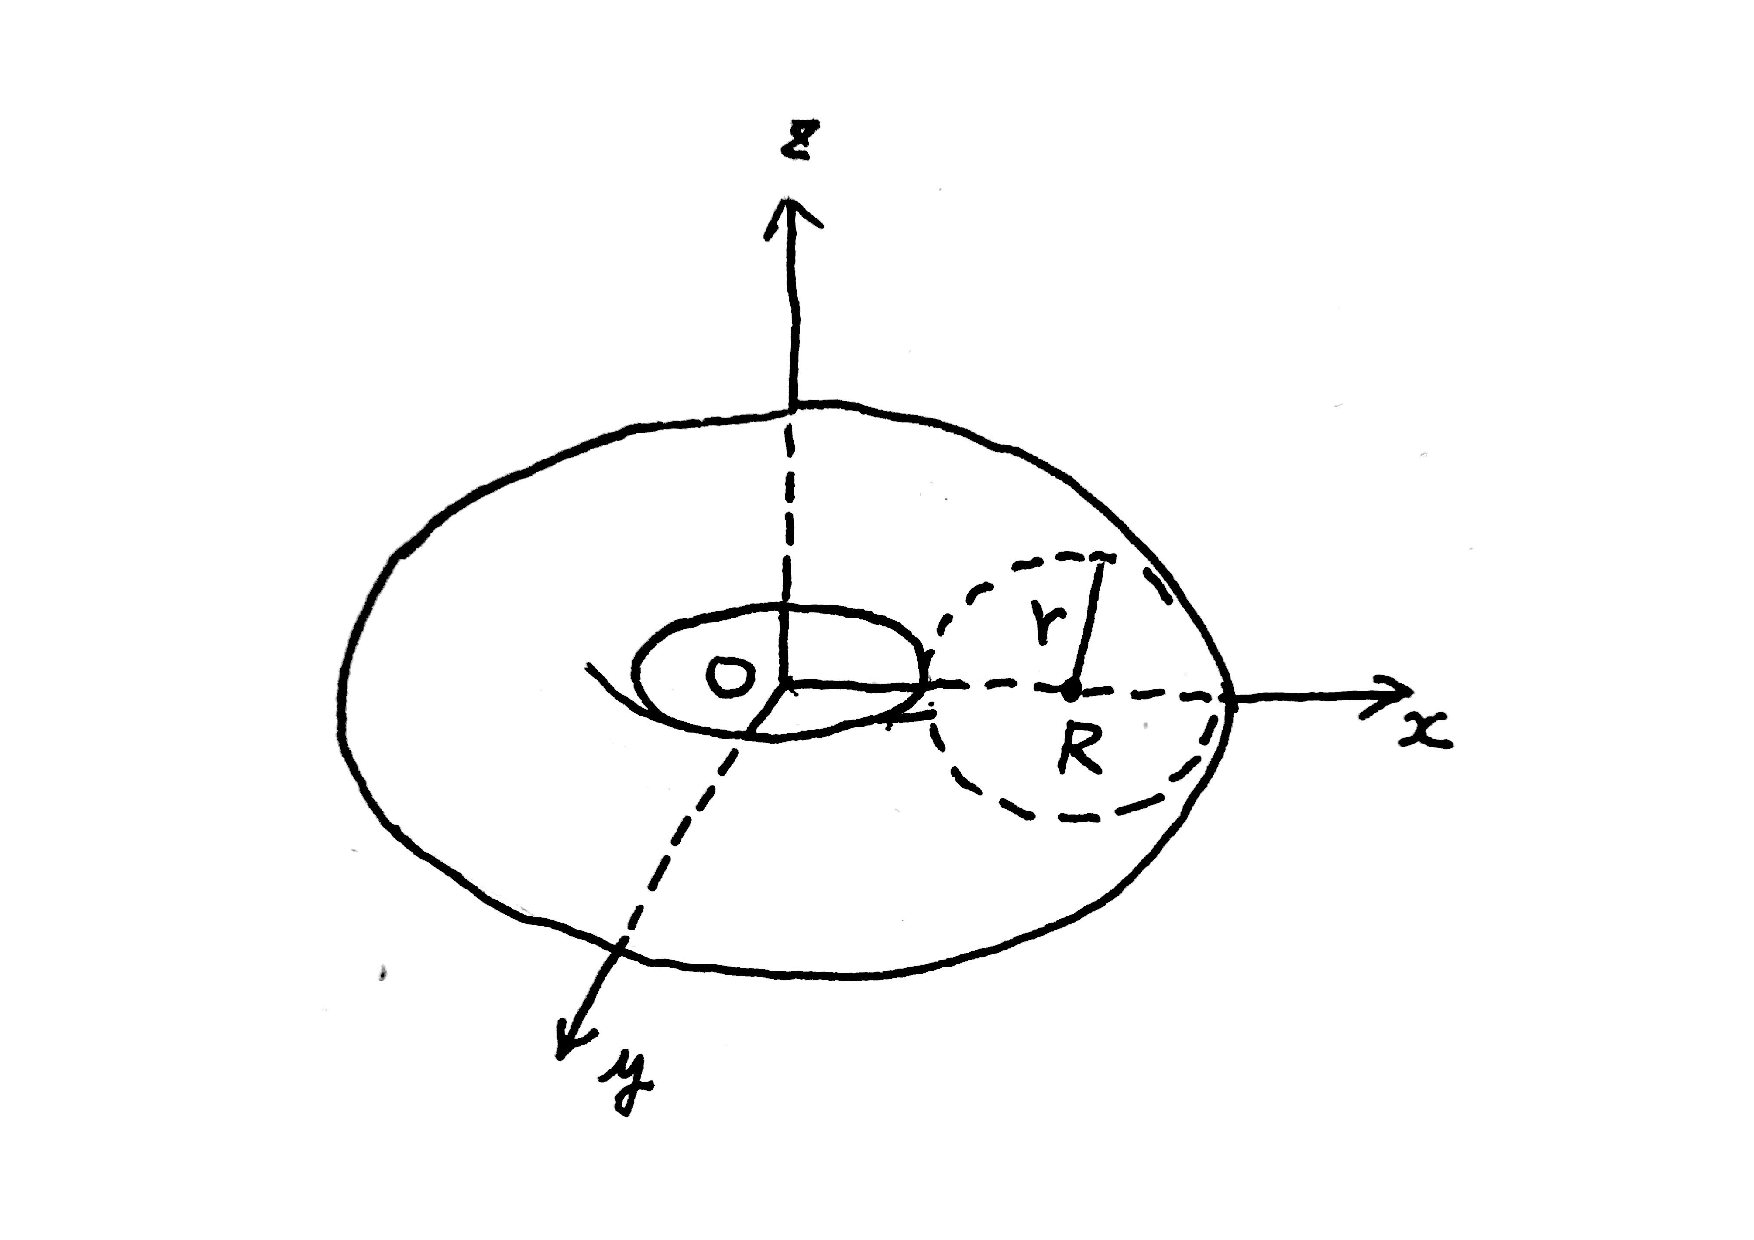
\includegraphics[keepaspectratio, scale=0.2]{T2Noshadow.pdf}
      \caption{$\mathbb{R}^3$の
      中の$2$次元トーラス$T^2$}
      \label{T2Noshadow}
     \end{figure}
\end{ex}
\end{frame}
\begin{frame}
    $C^\infty$級写像($C^\infty$級関数)
    $f:\mathbb{R}^3\to \mathbb{R}$
    を
    $$f(x,y,z)=(\sqrt{x^2+y^2}-R)^2+z^2-r^2$$
    と定義すると, 
    $$T^2=f^{-1}(0)$$
    となる. $\boldsymbol{p}=(x,y,z)$における
    ヤコビ行列
    $(Jf)_{\boldsymbol{p}}$を調べると, 
    であり, $\boldsymbol{p}\in T^2$のとき, 
    $$(Jf)_{\boldsymbol{p}}=
    \left(\frac{2(\sqrt{x^2+y^2}-R)x}
        {\sqrt{x^2+y^2}},\frac{2(\sqrt{x^2+y^2}-R)y}
        {\sqrt{x^2+y^2}},2z\right)\neq 
        \boldsymbol{o}$$
    となり, rank$(Jf)_{\boldsymbol{p}}=1$
    を得る. 
    したがって, $T^2$は$3-1=2$次元$C^\infty$
    級多様体である. 
\end{frame}
\begin{frame}
  \begin{ex}
    $2$次元トーラス$T^2=S^1\times S^1$は
    $2$次元$C^\infty$級多様体になる.  
  \end{ex}  
  $T^2=\{(x_1,x_2,x_3,x_4)\in \mathbb{R}^4|
  x_1^2+x_2^2=1, x_3^2+x_4^2=1\}$
  より, 
  $C^\infty$級写像$f:\mathbb{R}^4\to \mathbb{R}^2$
  を$f(x_1,x_2,x_3,x_4)=(x_1^2+x_2^2-1,
  x_3^2+x_4^2-1)$と定義すると, 
  $T^2=f^{-1}(0,0)$
  と表せる. ヤコビ行列$(Jf)_{\boldsymbol{x}}$は
  $$(Jf)_{\boldsymbol{x}}=
      \left(\begin{array}{cccc}
          2x_1&2x_2&0&0\\
          0&0&2x_3&2x_4
      \end{array}\right)$$
  $\boldsymbol{x}\in T^2$のとき, 
  rank$(Jf)_{\boldsymbol{x}}=2$であるから, 
  $T^2$は$4-2=2$次元$C^\infty$級
  多様体である.
\end{frame}

% \section{準備}
% \begin{frame}
% \frametitle{準備} 
% \begin{dfn}
% $(X, \mathcal{O})$, $(Y, \mathcal{O'})$を位相空間とする. 写像$f:X\rightarrow Y$が条件(1), (2)
% をみたすとき, $f$を同相写像という. \\
% (1)$f:X\rightarrow Y$は全単射である. \\
% (2)$f:X\rightarrow Y$も$f^{-1}:Y\rightarrow X$も, ともに連続写像である. \\
% 位相空間XとYの間に同相写像$f:X\rightarrow Y$があるとき, $X$と$Y$は互いに
% 位相同型であるといい, 記号で$X\approx Y$と表す. 
% \end{dfn}
% \begin{ex}
% 双曲線$xy=1$を$C$とすると, $C \approx \mathbb{R}/\{0\}$である. 
% \end{ex}
% \end{frame}

% \begin{frame}
% \begin{proof}
% $f:\mathbb{R}/\{0\}\rightarrow C$を$f(x)=(x, 1/x)$とすると, $f$は全単射
% かつ連続である. \\
% また, $f$の逆関数$f^{-1}$は$f^{-1}(x,y)=x$となり, これも連続である. 
% よって$f$は同相写像であるから, $C \approx \mathbb{R}/\{0\}$である. 
% \end{proof}
% \begin{tikzpicture}[scale=1.2]
%  \draw[blue] (0, 0, 0) circle (0.1);
% \draw[semithick, blue] (-2,0)--(-0.1,0);
% \draw[semithick] (-0.1,0)--(0.1,0);
% \draw[->,>=stealth,semithick, blue] (0.1,0)--(2,0); %x軸
% \draw[->,>=stealth,semithick] (0,-2)--(0,2) node[left]{$y$}; %y軸
% \draw (0,0) node[below left]{O}; %原点
% \draw [domain=0.5:2,samples=100,smooth, blue] plot (\x,{1/\x})node[right]{$xy=1$};
% \draw [domain=-2:-0.5,samples=100,smooth, blue] plot (\x,{1/\x});
% \draw[->](-1, 0)--(-1,-1)node[right]{$f$}; 

% \node at (2.3, 0) {$x$};
% \node at (1,-0.4) {\textcolor{blue}{$\mathbb{R}/\{0\}$}};
% \end{tikzpicture}
% \end{frame}



% \begin{frame}
% \frametitle{多様体の例} 
% \begin{dfn}
% $m$個の円周$S^1$の直積
% $$S^1 \times S^1 \times \cdots \times S^1$$
% を$m$次元トーラスといい, $T^m$と書く. 
% \end{dfn}
% \end{frame}

% \begin{frame}
% \frametitle{多様体の例} 
% \begin{thm}
% $2$次元トーラス$T^2$は$2$次元$\mathit{C}^\infty$級多様体である. \\
% \end{thm}

% $T^2$は$2$個の円周$S^1$の直積である. これは積位相を入れることで位相空間となり, 
% $S^1$の座標近傍$\mathcal{S}=\{(U_\alpha, \varphi_\alpha)\}_{\alpha \in A}$から導かれる
% 座標近傍\\
% $\{(U_\alpha \times U_\beta, \varphi_\alpha \times \varphi_\beta)\}_{\alpha , \beta \in A}$
% によって$2$次元$\mathit{C}^\infty$級多様体になる.\\
% \ \\
% \ \\
% \ \\
% \begin{tikzpicture}[scale=1.2]
%  \draw (4, 0) ellipse (1.5 and 1);
% \draw (3.2, 0.4+0.2) to[bend right] (4.8, 0.4+0.2);
% \draw (3.5, 0.2+0.2) to[bend left] (4.5, 0.2+0.2);
% \draw[line width=1pt,->] (4, -1) to[bend left] (4, 0.15);
% \draw[line width=1pt,->] (2.8, -0.2) to[bend right] (5.2, -0.2);
% \node at (5, 0)  {{\fontsize{9pt}{12pt}\selectfont $(U_\alpha \times U_\beta, \varphi_\alpha \times \varphi_\beta)$}};
% \node at (2.5, 0.75)  {$T^2$};
% \end{tikzpicture}
% \end{frame}

% \section{今後の目標}
% \begin{frame}
% \frametitle{今後の目標} 
% 現在は, 射影平面$P^2$はメビウスの帯と円盤を貼り合わせたものであるという定性的な
% 理解に留まっているが, これから$P^2$の厳密な定義と, 「はめ込み」, 「埋め込み」の定義を学び, $\mathbb{R}^3$へのはめ込み可能性と埋め込み可能性を調べていきたい.\\
% \ \\
% \ \\
% \ \\
% \begin{tikzpicture}

% \draw[line width=1pt,->] (-0.75,0.75) to[bend right](1, 0.4);
% \draw[line width=1pt,->] (1,0.4) to[bend right](-0.2, 0.4);
% \draw[dashed] (-0.3, 0.4) to[bend right](-0.75,0);
% \draw[line width=1pt,->](-0.75,0) to[bend right](1.5, 0.4);
% \draw[line width=1pt,->](1.5, 0.4) to[bend right](-0.75,0.75);
% \draw[line width=1pt] (-0.75,0.75) to[bend right](-0.75,0);
% \node at (0, -0.8)  {メビウスの帯};
% \pause
% \node at (2+0.5, 0.3)  {$+$};
% % 球面の描画
%     \draw[line width=1pt,->] (3+1.5, 0.3) circle (0.7);
%     \draw[line width=1pt] (3.1+1.5, 1.1) -- (3+1.5, 1);
%     \draw[line width=1pt] (3.1+1.5, 0.9) -- (3+1.5, 1);
% \node at (3+1.5, -0.8)  {円盤};
% \pause

% \draw[line width=1pt, ->] (4+2, 0.3) -- (5+4, 0.3);
% \node at (4.5+3, -0.3)  {線に沿って貼り合わせる};
% \node at (4.7+3, -0.8)  {\textcolor{red}{($\mathbb{R}^3$内だと難しい)}};
% \node at (6+4, 0.3)  {{\fontsize{12pt}{12pt}\selectfont $P^2$}};
% \end{tikzpicture}
% \ \\
% (参考文献\cite{Matsumoto18}参照)
\begin{frame}
    \frametitle{おわりに}
  空間を多様体$M$, $N$の間の$C^r$級写像$f:M\to N$の逆像$f^{-1}(q)$
(ただし$q$は$N$のある$1$点)
とみなせれば, $f$のヤコビ行列の階数を計算することで
多様体としての次元を調べることができるという
ことが分かった. 

今後の課題としては, 多様体が
部分多様体として実現できる空間の
条件(埋め込み可能性)について調べたい. 
\end{frame}

\begin{frame}
\frametitle{参考文献} 
\begin{thebibliography}{1}
\beamertemplatetextbibitems
\bibitem{Matsumoto18} 松本幸夫, [第30版]多様体の基礎, 東京大学出版会, 2018.
  \bibitem{Hujioka17} 藤岡敦, [第2版]具体例から学ぶ 多様体, 裳華房, 2017.
  \bibitem{Hattori76} 服部晶夫, [第1版]多様体, 岩波書店, 1976.
\end{thebibliography}
\end{frame}

\end{document}